\documentclass[11pt]{article}


\usepackage{fullpage}
\usepackage{graphicx}
\usepackage{amsmath}
\usepackage{amssymb}
\usepackage{amsthm}
\usepackage{fancyvrb}

\newcommand{\myname}{Mehshan Mustafa}

\newenvironment{theorem}[2][Theorem]{\begin{trivlist}
\item[\hskip \labelsep {\bfseries #1}\hskip \labelsep {\bfseries #2.}]}{\end{trivlist}}
\newenvironment{lemma}[2][Lemma]{\begin{trivlist}
\item[\hskip \labelsep {\bfseries #1}\hskip \labelsep {\bfseries #2.}]}{\end{trivlist}}
\newenvironment{exercise}[2][Exercise]{\begin{trivlist}
\item[\hskip \labelsep {\bfseries #1}\hskip \labelsep {\bfseries #2.}]}{\end{trivlist}}
\newenvironment{problem}[2][Problem]{\begin{trivlist}
\item[\hskip \labelsep {\bfseries #1}\hskip \labelsep {\bfseries #2.}]}{\end{trivlist}}
\newenvironment{question}[2][Question]{\begin{trivlist}
\item[\hskip \labelsep {\bfseries #1}\hskip \labelsep {\bfseries #2.}]}{\end{trivlist}}
\newenvironment{corollary}[2][Corollary]{\begin{trivlist}
\item[\hskip \labelsep {\bfseries #1}\hskip \labelsep {\bfseries #2.}]}{\end{trivlist}}
\newenvironment{solution}{\begin{proof}[Solution]}{\end{proof}}
\newenvironment{idea}[2][Proof Idea.]{\textit{#1} #2}



\parindent0in
\pagestyle{plain}
\thispagestyle{plain}

\newcommand{\dated}{\today}
\newcommand{\token}[1]{\langle \text{#1} \rangle}

\begin{document}

\textbf{Introduction to the Theory of
Computation}\hfill\textbf{\myname}\\[0.01in]
\textbf{Chapter 2: Context-Free Languages}\hfill\textbf{\dated}\\
\smallskip\hrule\bigskip

\begin{problem}{2.27}
Let $G = (V, \Sigma, R, \langle$STMT$\rangle)$ be the following grammar.
\begin{center}
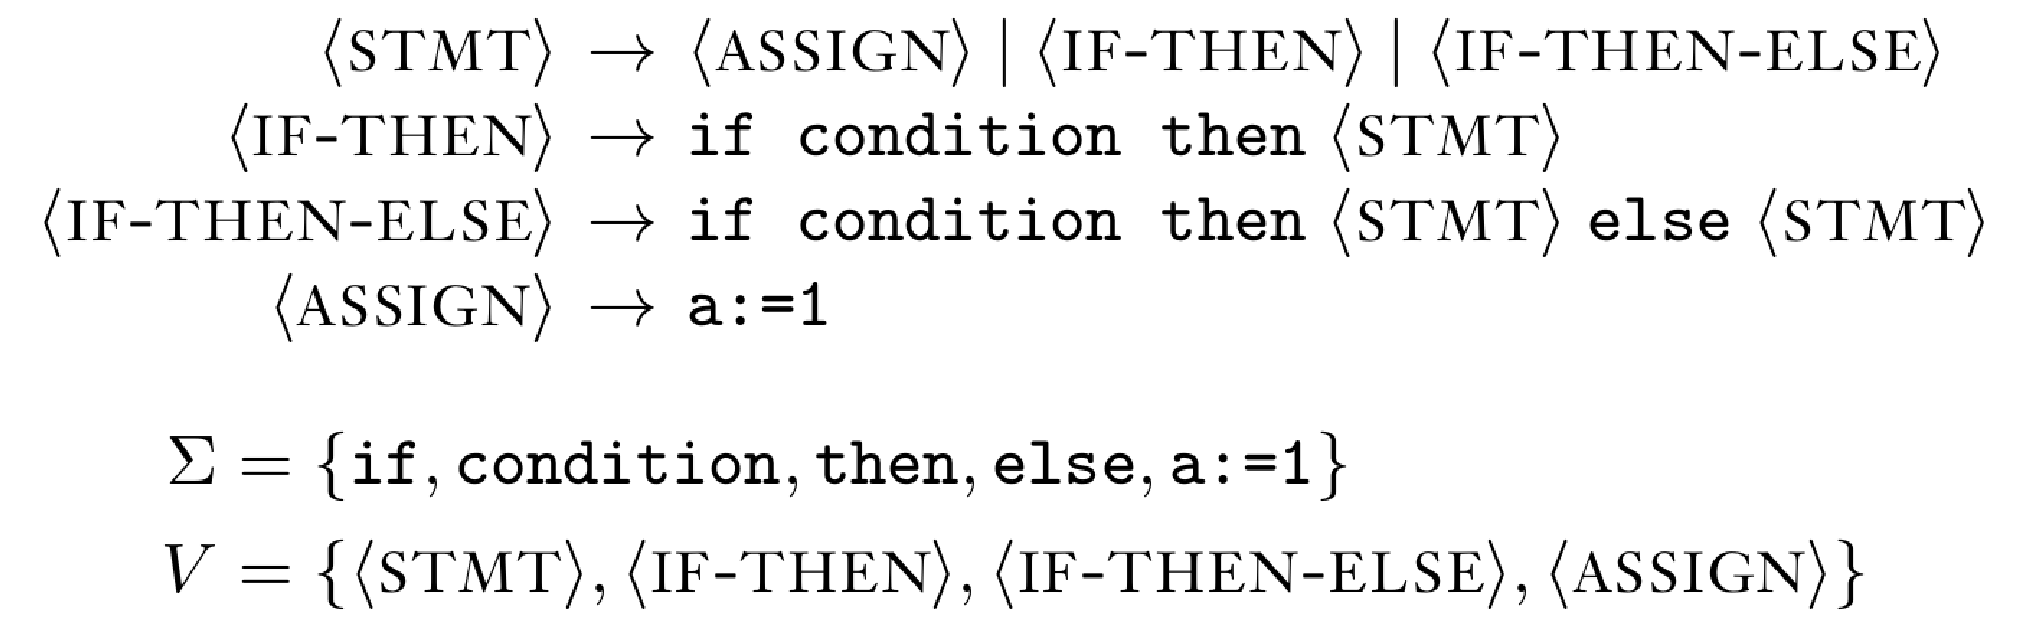
\includegraphics[scale=0.4]{Figures/Problem2.27a.pdf} \\
\end{center}
$G$ is a natural-looking grammar for a fragment of a programming language, but $G$ is ambiguous.
\end{problem}

\begin{problem}[Part]{a}
Show that $G$ is ambiguous.
\end{problem}

The string ``if condition then if condition then a:=1 else a:=1" has two different parse trees in $G$.
\begin{center}
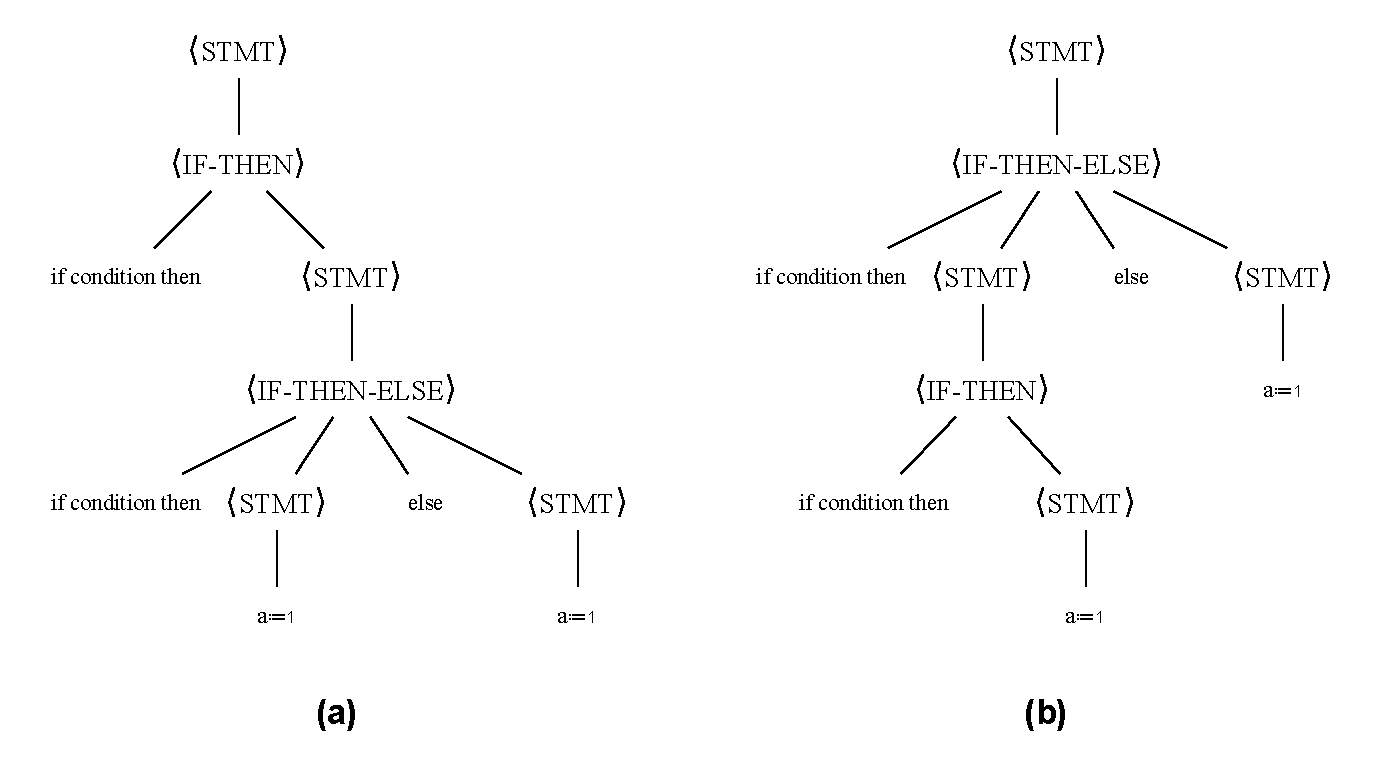
\includegraphics[scale=0.7]{Figures/Problem2.27b.pdf} \\
Two different parse trees of the string \\
``if condition then if condition then a:=1 else a:=1".
\end{center}

\newpage 

\begin{problem}[Part]{b}
Give a new unambiguous grammar for the same language.
\end{problem}
\begin{align*}
\token{STMT} &\rightarrow \token{ASSIGN} \ | \ \token{IF-THEN} \\
\token{IF-THEN} &\rightarrow \text{if condition then} \ \token{IF-BODY} \\
\token{IF-BODY} &\rightarrow \token{ASSIGN} \ | \ \token{IF-THEN} \ | \ \token{ASSIGN} \ \token{ELSE} \\
\token{ELSE} &\rightarrow \text{else} \ \token{ELSE-BODY} \\
\token{ELSE-BODY} &\rightarrow \token{ASSIGN} \ | \ \token{IF-THEN} \\
\token{ASSIGN} &\rightarrow \text{a:=1} \\
\end{align*}

\end{document}
